\FloatBarrier
\section{Durchführung}
\label{sec:Durchführung}

Um die Suszeptibilität paramagnetischer Stoffe experimentell bestimmen zu können, wird eine Brückenschaltung verwendet.
Der Aufbau dieser ist in Abbildung \ref{fig:Brückenschaltung} dargestellt.
Wie in Abschnitt \ref{sec:praktischeTheorie} beschrieben, sind die bei diesem Aufbau auftretenden Brückenspannungen in der Größenordnung der Störspannungen.
Es sind daher einige Maßnahmen nötig um die Brückenspannungen auswerten und somit die Suszeptibilität ausrechnen zu können.
Der grobe Aufbau ist in Abbildung \ref{fig:Aufbau} gezeigt.

\begin{figure}
  \centering
  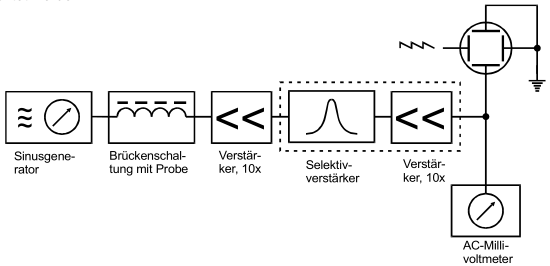
\includegraphics[width=0.75\textwidth]{images/Aufbau.png}
  \caption{Maßnahmen, um die Brückenspannung vernünftig isolieren zu können, entnommen der Versuchsanleitung\cite[183]{sample}}
  \label{fig:Aufbau}
\end{figure}

 Am wichtigsten zum Isolieren der Brückenspannung ist der bereits erwähnte Selektivverstärker.
 Er ermöglicht es die monofrequente Brückenspannung aus der breitbandigen Störspannung hinreichend genau zu isolieren.
 Eine beispielhafte Filterkurve ist in Abbildung \ref{fig:theofilterkurve} dargestellt.
 Die dort erwähnte Güte gibt die entsprechende Weite der Kurve an.
 Diese wird für diesen Versuch auf $\text{Q} = 100$ eingestellt.

 Die Filterkurve wird zur Verifizierung dieses Wertes untersucht.
 Dafür wird ein Synthesizer direkt mit dem Selektivverstärker verbunden.
 Die Durchlassfrequenz des Selektivverstärker wird auf einen Wert zwischen $30 - \SI{40}{\kilo\hertz}$ eingestellt.
 Bei konstanter Eingangsspannung von maximal $\SI{1}{\volt}$ wird dann die Ausgangsspannung in Abhängigkeit von der Frequenz zwischen $30 - \SI{40}{\kilo\hertz}$ gemessen.

Zur Bestimmung der eigentlichen Suszeptibilität werden die Elemente gemäß Abbildung \ref{fig:Aufbau} aufgebaut.
Der Sinusgenerator wird auf die Frequenz eingestellt, für die der Selektivverstärker ein Maximum besitzt.
Die Spannung beträgt dabei $\SI{1}{\volt}$.
Der Sinusgenerator wird mit der Brückenschaltungen verbunden.
Die so entstehende Brückenspannung wird abgegriffen und durch einen Linearverstärker $10\times$ vorverstärkt.
Diese wird nun durch den Selektivverstärker gefiltert und durch ein Millivoltmeter gemessen.
Um den Selektivverstärker mit dem Sinusgenerator zu eichen, wird die Ausgangsspannung bei einer Güte $\text{Q} = 100$ auf ihren Maximalwert eingestellt, indem die Durchlassfrequenz des Selektivverstärkers variiert wird.

Anschließend wird die Brückenschaltung ohne Probe abgeglichen, indem der Widerstand R$_3$ und R$_4$ so eingeregelt wird, dass die gemessene Brückenspannung minimal wird.
Die Spannung und der Wert des Widerstandes wird notiert.
Sogleich wird die Probe in die Spule L$_\text{M}$ (s.h. Abbildung \ref{fig:Brückenschaltung}) eingeführt.
Die gemessene Spannung sollte sich nun ändern und notiert werden.
Die Widerstände R$_3$ und R$_4$ werden erneut auf das Spannungsminimum eingestellt.
Es ist hierbei darauf zu achten, dass die Proben nicht zu lange in der Hand gehalten werden, da diese sich sonst erhitzen und die geänderte Temperatur den sehr wärmeempfindlichen Wert der Suszeptibilität verfälschen würden.
Diese Messungen werden jeweils dreimal für drei unterschiedliche Proben, Neodym(III)-oxid, Gadolinium(III)-oxid und Dysprosium(III)-oxid, durchgeführt.
Zuletzt werden noch die Massen der Proben abgelesen und deren Länge mit einem Lineal bestimmt.
